\section{Kiến thức chuẩn bị}

Trong mục này, chúng tôi trình bày một số kiến thức chuẩn bị cho các nội dung được nghiên cứu trong các phần sau.

\begin{comment}
    \section{Hàm Gauss}
    Hàm Gauss là một hàm số có dạng cơ sở là:
    \[
        f(x) = \exp \left( -x^2 \right), 
    \]
    
    và có dạng tham số là:
    \[
        f(x) = a \exp \left(- \dfrac{1}{2} \dfrac{(x-b)^2}{c^2}\right),
    \]
    
    với tham số $a$ là độ cao, $b$ là vị trí của đỉnh, và $c$ điều khiển độ rộng của đồ thị hàm số.
    
    Trong xác suất thống kê, hàm Gauss thường được dùng để biểu diễn cho hàm mật độ xác suất của phân phối chuẩn:
    \[
        f(x) = \dfrac{1}{\sigma \sqrt{2\pi}} \exp \left( -\dfrac{1}{2} \dfrac{(x-\mu)^2}{\sigma^2} \right),
    \]
    với $\mu$ là trung bình và $\sigma^2$ là phương sai của phân phối.
    
    % Ngoài ra, ta còn có thể viết dưới dạng
    % \[
    %     f(x) = \dfrac{1}{\sigma \sqrt{2\pi}} \exp \left( -\dfrac{1}{2} \dfrac{(x-\mu)^2}{\sigma^2} \right),
    % \]    
\end{comment}



\subsection{Phân phối chuẩn đa biến}
Phân phối chuẩn đa biến $X \sim \Normal(\mu, \cov)$ với vector trung bình là $\mu \in \R^d$ và ma trận hiệp phương sai đối xứng, nửa xác định dương $\cov \in \R^{d \times d}$, có 
% pdf 
hàm mật độ xác suất
như sau:
\[
    f(x | \mu, \cov) 
    % \Normal(x | \mu,\cov)
    % f_X(x)
    = \frac{1}{\sqrt{(2\pi)^{d} |\cov|}}  \exp \left(- \frac{1}{2} (x - \mu)^{T} \cov^{-1}  (x - \mu)\right), \ x \in \R^d,
\]
với $|\cov|$ là định thức của $\cov$.

% \begin{draft}
\textbf{Lý do sử dụng phân phối chuẩn đa biến cho bài toán xử lý dữ liệu khuyết?}

\begin{itemize}
    \item Nhiều phương pháp thống kê dựa trên giả định dữ liệu có phân phối chuẩn, dễ làm việc hơn vì được nghiên cứu lâu dài, cùng với Định lý giới hạn trung tâm khiến cho phân phối chuẩn được sử dụng rộng rãi.
    \item Dữ liệu thực tế thường có nhiều cột đặc trưng (features), dẫn đến dữ liệu có số chiều cao, nên ta cần một phân phối có khả năng xử lý dữ liệu nhiều chiều và cho ta thấy được mối tương quan giữa các đặc trưng với nhau.
    \item Phân phối chuẩn đa biến cho phép mô hình hoá các phân phối xác suất đồng thời của các đặc trưng khác nhau.
    % (?)
\end{itemize}
% \end{draft}

Trong khuôn khổ bài báo cáo này, từ giờ về sau, hàm mật độ xác suất của phân phối chuẩn đa biến sẽ được gọi là hàm Gauss để cho thuận tiện.

\begin{lemma}\label{lem:prod_gauss} (Tích của hai hàm Gauss là một hàm Gauss)

    Cho $f(x) = \exp\left(-\dfrac{1}{2}(x - a)^{\top} A^{-1} (x - a)\right)$ 
    và $g(x) = \exp\left( -\dfrac{1}{2} (x - b)^{\top} B^{-1} (x - b)\right)$ là hai hàm Gauss, với $A$ và $B$ là ma trận nửa xác định dương, ta có:
    \[
        f(x)g(x)=\exp\left(-\frac{1}{2}(a-b)^{\top}(A+B)^{-1}(a-b)\right)
        \exp\left(-\frac{1}{2}(x-\mu_{p})^{\top}\cov_{p}^{-1}(x-\mu_{p})\right),
    \]
    với $\mu_p$ và $\cov_p$ 
    lần lượt là vector trung bình và ma trận hiệp phương sai của tích hai hàm Gauss, 
    phụ thuộc vào $a$, $A$, $b$, và $B$.
\end{lemma}

\begin{proof}
    % Phần chứng minh của bổ đề này có thể tìm thấy ở trong 
    Xem mục A.2 trong bài báo \cite{le2020neumiss}.
\end{proof}

\begin{comment}
\begin{proof}
    Với $f(X)$ có phân phối chuẩn đa biến $\Normal(X | a, A)$, ta có:
    \begin{align*}
        f(X) &= \exp\left(-\dfrac{1}{2}(X - a)^{\top} A^{-1} (X - a)\right) \\
        % &= \exp((X - a)^{\top} (A^{-1}X - A^{-1}a )) \\
        &= \exp\left(-\dfrac{1}{2}(X^{\top}A^{-1}X - X^{\top}A^{-1}a - a^{\top} A^{-1}X + a^{\top}A^{-1}a) \right)\\
        &= \exp\left( -\dfrac{1}{2}(X^{\top}A^{-1}X - 2X^{\top}A^{-1}a + a^{\top}A^{-1}a) \right).
    \end{align*}
    Qua đây, ta thấy được $A^{-1}$ là nghịch đảo của phương sai, $A^{-1}a$ là tích của nghịch đảo phương sai với trung bình của $X$, và $a^{\top}A^{-1}a$ là hằng số. Tiếp theo ta sẽ thấy được sự tương đồng đối với trường hợp $f(X)g(X)$.
    
    Ta xét:
    \begin{align}
        f(X)g(X) &= \exp\left(-\dfrac{1}{2}(X - a)^{\top} A^{-1} (X - a)\right) \exp\left(-\dfrac{1}{2}(X - b)^{\top} B^{-1} (X - b)\right) \notag \\
        &= \exp\left(-\dfrac{1}{2}\left((X - a)^{\top} A^{-1} (X - a) + (X - b)^{\top} B^{-1} (X - b)\right) \right) \notag \\
        &= \exp\left(-\dfrac{1}{2}\left( X^{\top}A^{-1}X - 2X^{\top}A^{-1}a + a^{\top}A^{-1}a + 
        X^{\top}B^{-1}X - 2X^{\top}B^{-1}b + b^{\top}B^{-1}b\right) \right) \notag \\
        &= \exp\left( -\dfrac{1}{2} \left(X^{\top}(A^{-1} + B^{-1})X - 2X^{\top}(A^{-1}a + B^{-1}b) + a^{\top}A^{-1}a + b^{\top}B^{-1}b \right) \right). \label{eq:fxgx}
    \end{align}
    Với $\mu_p$ và $\cov_p$ 
    lần lượt là vector trung bình và ma trận hiệp phương sai của tích hai hàm Gauss, ta đặt:
    \begin{align*}
        \cov_{p}^{-1} &= A^{-1} + B^{-1}, \\
        \cov_{p}^{-1} \mu_p &= A^{-1}a + B^{-1}b.
    \end{align*}
    Thay vào \eqref{eq:fxgx}, ta có:
    \begin{align*}
        f(X)g(X) &= \exp \left( -\dfrac{1}{2} \left(X^{\top}\cov_p^{-1}X - 2X^{\top}\cov_p^{-1} \mu_p + a^{\top}A^{-1}a + b^{\top}B^{-1}b\right) \right) \\
        &= \exp \left( -\dfrac{1}{2} \left(X^{\top}\cov_p^{-1}X - 2X^{\top}\cov_p^{-1} \mu_p + \mu_{p}^{\top} \cov_p^{-1}\mu_p - \mu_{p}^{\top} \cov_p^{-1}\mu_p  + a^{\top}A^{-1}a + b^{\top}B^{-1}b\right) \right) \\
        &= \exp\left( -\dfrac{1}{2} \left(X^{\top}\cov_p^{-1}X - 2X^{\top}\cov_p^{-1} \mu_p + \mu_{p}^{\top} \cov_p^{-1}\mu_p \right) \right) \\
         &\quad \quad \times \exp\left( -\dfrac{1}{2} \left(a^{\top}A^{-1}a + b^{\top}B^{-1}b - \mu_{p}^{\top} \cov_p^{-1}\mu_p \right) \right)\\
        &= \exp\left( -\dfrac{1}{2}\left(a^{\top}A^{-1}a + b^{\top}B^{-1}b - \mu_{p}^{\top} \cov_p^{-1}\mu_p \right) \right) \exp\left( -\dfrac{1}{2} (X-\mu_p)^{\top}\cov_p^{-1}(X - \mu_p)\right).
    \end{align*}
    Giờ ta đi đơn giản phần hệ số ở phía trước:
    \begin{align}
        c &= a^{\top}A^{-1}a + b^{\top}B^{-1}b - \mu_{p}^{\top} \cov_p^{-1}\mu_p \notag \\
        &= a^{\top}A^{-1}a + b^{\top}B^{-1}b - 
        \left(a^{\top}A^{-1}(A^{-1}+B^{-1})^{-1}+b^{\top}B^{-1}(A^{-1}+B^{-1})^{-1}\right) (A^{-1}a + B^{-1}b) \notag \\
        &= a^{\top}(A^{-1}-A^{-1}(A^{-1} + B^{-1})^{-1}A^{-1})a+b^{\top}(B^{-1}-B^{-1}(A^{-1}+B^{-1})^{-1}B^{-1})b \notag \\
        &\quad \quad -2a^{\top} (A^{-1} (A^{-1} + B^{-1})^{-1} B^{-1} )b.
        % \quad \quad \quad \text{(Do } A \text{ và } B \text{ đối xứng)} 
        \label{eq:need_woodbury}
    \end{align}
    Ta có Woodbury Identity (Đồng nhất thức Woodbury) cho các ma trận có thể nhân hoặc cộng được với nhau (conformable) $A, B, C, D$ dưới dạng:
    \[
        \displaystyle \left(A+CBD\right)^{-1} = A^{-1}-A^{-1}C\left(B^{-1}+DA^{-1}C\right)^{-1}DA^{-1}.
    \]
    Việc khai triển phương trình trên có thể tìm thấy ở \cite{ridgway2006matrixwoodbury}. Khi $C = D = I$, ta được:
    \[
        \left(A+B\right)^{-1}=A^{-1}-A^{-1}\left(B^{-1}+A^{-1}\right)^{-1}A^{-1}.
    \]
    Thay vào \eqref{eq:need_woodbury}, ta được
    \begin{align*}
        c &= a^{\top} (A+B)^{-1} a + b^{\top}(A + B)^{-1}b 
        -2a^{\top} (A^{-1} (A^{-1} + B^{-1})^{-1} B^{-1} )b \\
        &= a^{\top} (A+B)^{-1} a + b^{\top}(A + B)^{-1}b -2a^{\top} \left(B(A^{-1} + B^{-1})A \right)^{-1}b \\
        &= a^{\top} (A+B)^{-1} a + b^{\top}(A + B)^{-1}b -2a^{\top} \left(BA^{-1}A + BB^{-1}A \right)^{-1}b \\
        &= a^{\top} (A+B)^{-1} a + b^{\top}(A + B)^{-1}b -2a^{\top} \left(B + A \right)^{-1}b \\
        &= (a-b)^{\top} (A+B)^{-1} (a-b).
    \end{align*}
    Vậy 
    \[
        f(X)g(X) = \exp\left(-\dfrac{1}{2}(a-b)^{\top} (A+B)^{-1} (a-b)\right) 
        \exp\left(-\dfrac{1}{2}(X-\mu_p)^{\top}\cov_p^{-1}(X - \mu_p)\right) \qed
    \]
\end{proof}
\end{comment}


\subsection{Phân phối chuẩn có điều kiện}
Một tính chất quan trọng của phân phối chuẩn đa biến đó là nếu $2$ tập hợp biến ngẫu nhiên có phân phối chuẩn đa biến đồng thời (Joint Gaussian), thì phân phối có điều kiện của một tập khi biết tập còn lại cũng là một phân phối chuẩn đa biến, tức 
\[
    f(x_a | x_b) = \Normal(x_a | \mu_{a|b}, \cov_{a|b}).
\]

Giả sử $x$ là vector $d$ chiều có phân phối chuẩn đa biến $\Normal(x|\mu, \cov)$. Ta chia $x$ thành $2$ tập con riêng biệt $x_a$ và $x_b$ được cho bởi \[
x = \begin{pmatrix}
    x_a \\
    x_b
\end{pmatrix}.
\]
Lúc này $x$ cũng được gọi là phân phối chuẩn đa biến bị chia  (Partitioned Multivariate Gaussian).
Ta cũng định nghĩa vector trung bình 
\[
\mu = \begin{pmatrix}
    \mu_a \\
    \mu_b
\end{pmatrix},
\]
và ma trận hiệp phương sai 
\[
\cov = \begin{pmatrix}
    \cov_{aa} & \cov_{ab} \\
    \cov_{ba} & \cov_{bb} \\
\end{pmatrix}.
\]

Ta có: 
\[
    \begin{split}
        \mu_{a|b} &= \mu_a + \cov_{ab}\cov_{bb}^{-1} (x_b - \mu_b), \\ 
        \cov_{a|b} &= \cov_{aa} - \cov_{ab} \cov_{bb}^{-1} \cov_{ba}.
    \end{split}
\]

\begin{proof}
    Xem mục 2.3.1 của \cite{bishop2006pattern} hoặc \cite{statexconditionalgaussian}. \qed
\end{proof}

Ngoài ra, nếu ma trận hiệp phương sai $\cov_{ab} = 0$, ta có $\mu_{a|b} = \mu_a$, $\cov_{a|b} = \cov_{aa}$, tức $x_a$ và $x_b$ độc lập với nhau, với $P(x_a|x_b) = P(x_a)$. Tức là khi ta lấy tích của các biến ngẫu nhiên độc lập với nhau, ta chỉ cần lấy các phần tử đường chéo của ma trận hiệp phương sai $\cov$.


\subsection{Chuẩn ma trận (Induced vector norm)}
Với chuẩn $2$ của vector $x = (x_1, \dots, x_n) \in \R^n$ có dạng:
\[
    \|x\|_2 = \sqrt{ \sum_{i=1}^n x_{i}^2}
    = \sqrt{x^{\top} x}
    = \sqrt{\langle x, x \rangle},
\] ta xét chuẩn 2 (induced-2 norm) cho ma trận $A$, hay còn được biết đến là chuẩn phổ (spectral norm):
\[
    \|A\|_2 = \max_{x \neq 0} {\frac{\|Ax\|_2}{\|x\|_2}}
    = \max_{\substack{x \neq 0 \\ \|x\|_2 = 1}} {\|Ax\|_2} = 
    \sigma_{max} (A),
\]

với $\sigma_{max} (A)$ là giá trị suy biến (singular value) lớn nhất của $A$. Và khi $A$ đối xứng, xác định dương, thì giá trị suy biến tương ứng với lại trị riêng của ma trận, tức $\|A\|_2 = \lambda_{\max}$.


\subsection{Chuỗi Neumann}
Chuỗi Neumann thường làm việc với các toán tử trong các không gian hàm. Nhưng trong khuôn khổ bài báo cáo, ta chỉ cần làm việc với ma trận -- toán tử biến đổi tuyến tính.

Với ma trận $A \in \R^{d \times d}$, chuỗi Neumann của $A$ được biểu diễn dưới dạng
\begin{equation*}
    \sum_{k=0}^{\infty} A^k = I + A + A^2 + \dots,
\end{equation*}
với $I$ là ma trận đơn vị.
Chuỗi Neumann hội tụ với điều kiện chuẩn phổ 
của ma trận $A$ bé hơn $1$ ($\|A\|_2 < 1$).
Và khi chuỗi hội tụ, tồn tại nghịch đảo của $(I - A)$ với:
\begin{equation*}
    (I - A)^{-1} = \sum_{k=0}^{\infty} A^k.
\end{equation*}

Để chứng minh điều trên, ta xét:
\[
    S_n = \sum_{k=0}^n A^k.
\]

Ta có:
\[
    \lim_{n \to \infty }(I - A) S_{n}
    =\lim_{n \to \infty} \left(\sum_{k=0}^{n}A^{k} - \sum_{k=0}^{n}A^{k+1}\right)
    =\lim_{n \to \infty} \left(I-A^{n+1}\right) = I.
\]
Vậy nghịch đảo của $I-A$ là chuỗi Neumann của $A$.

Từ đây, chuỗi Neumann có thể được sử dụng để xấp xỉ nghịch đảo của một ma trận: Xét ma trận $A$ khả nghịch, ta có:
\begin{equation*}
    \begin{split}
        A^{-1} &= (I - I + A)^{-1}\\
        &= (I - (I - A))^{-1}\\
        &= (I - T)^{-1}, \\
    \end{split}
\end{equation*}
với $T = I - A$. Nếu $T$ thoả điều kiện $\|T\|_2 < 1$, thì ta có theo chuỗi Neumann:
\[
    (I - T)^{-1} = \sum_{k=0}^{\infty} T^k.  
\]
Và do đó:
\begin{equation*}
    A^{-1} = (I - (I - A))^{-1} = \sum_{k=0}^{\infty} (I - A)^k.
\end{equation*}

Vì với điều kiện $\|I-A\|_2 < 1$, $I-A$ dần hội tụ khi $k \to \infty$, nên chuỗi chặt cụt (truncated) tại $l$ hữu hạn có thể cho ta 1 xấp xỉ nghịch đảo ma trận tốt.
\begin{equation*}
     A^{-1} \approx \sum_{k=0}^{l}(I-A)^{k}.
\end{equation*}



\subsection{Bán kính phổ}
Cho ma trận $A \in \C^{d \times d}$ với các trị riêng $\lambda_1, \dots, \lambda_d$, bán kính phổ (spectral radius) $\rho (A)$ của $A$ là giá trị tuyệt đối trị riêng lớn nhất của ma trận $A$:
\[
    \rho (A) = \max\{|\lambda_1|, \dots, |\lambda_d|\}.
\]

Khi $A$ là ma trận thực đối xứng, bán kính phổ của $A$ bằng với chuẩn phổ của $A$:
\[
    \rho (A) = \|A\|_2 = \lambda_{\max}.
\]

\subsection{Tỷ số Rayleigh (Rayleigh quotient)}
Tỷ số Rayleigh thường được sử dụng để xấp xỉ trị riêng của ma trận thực đối xứng $A$ dưới dạng: 
\[
    r(x) = \dfrac{x^{\top} A x}{x^{\top} x},
\]
với $x \neq 0$.

Để cho đơn giản, ta cho $\|x\| = 1$, lúc này, việc tìm trị riêng lớn nhất của $A$ có dạng:
\[
    \lambda_{\max}(A) = \rho(A) =  \max_{\substack{\|x\|=1}} x^{\top} A x.
\]


Người đọc có thể đọc thêm về phần kiến thức này ở phần \MakeUppercase{\romannumeral 5} trong \cite{trefethennumerical}.


% \section{Law of total expectation (Luật kỳ vọng đầy đủ)}
% Law of total expectation (hay Law of iterated expectation) cho ta biết rằng kỳ vọng của một biến ngẫu nhiên bằng với lại tổng các kỳ vọng của biến ngẫu nhiên đó dựa trên một biến ngẫu nhiên khác. 

% Với biến ngẫu nhiên $X$, $Y$, ta có
% \[
%     \E\left[\E[X|Y]\right] = \E [X].
% \]



\subsection{Phép nhân Hadamard (Hadamard product)}
Trong các phép toán ma trận, phép nhân Hadamard, ký hiệu là $\odot$, là phép nhân từng phần tử (element-wise) của 2 ma trận với nhau. 

Xét $A \in \R^{m \times n}$ và $B \in \R^{m \times n}$, với lần lượt $a_{ij}$, $b_{ij}$ nằm ở dòng thứ $i$ và cột thứ $j$ của ma trận $A$, $B$. Phép nhân Hadamard của ma trận $A$ và $B$ là:
\[
    \mathbf{A} \odot \mathbf{B} =
    \begin{bmatrix}
        a_{11}  b_{11} & a_{12}  b_{12} & \dots  & a_{1n}  b_{1n} \\
        a_{21}  b_{21} & a_{22}  b_{22} & \dots  & a_{2n}  b_{2n} \\
        \vdots & \vdots & \ddots & \vdots \\
        a_{m1}  b_{m1} & a_{m2}  b_{m2} & \dots  & a_{mn}  b_{mn}
    \end{bmatrix}.
\]


\subsection{Điểm bất động}
Điểm bất động (fixed point) $x^*$ là điểm thoả 
\[
    f(x^*) = x^*,
\]
với hàm $f$ cố định. Nói cách khác, điểm bất động là điểm không thay đổi với 1 phép biến đổi cho trước.


\subsection{Algorithm Unrolling}
Ý tưởng của Algorithm Unrolling được giới thiệu lần đầu trong công trình của Gregor và LeCun \cite{gregor2010unroll}, nhằm liên kết các thuật toán lặp (Iterative algorithms) với các neural networks. Cụ thể, mỗi vòng lặp trong thuật toán được mô hình hóa như một lớp (layer) trong mạng, qua đó thuật toán lặp được biểu diễn như một chuỗi các lớp liên tiếp. Việc truyền qua mạng tương đương với việc thực thi thuật toán lặp một số lần hữu hạn.

\begin{figure}[h]
    \centering
    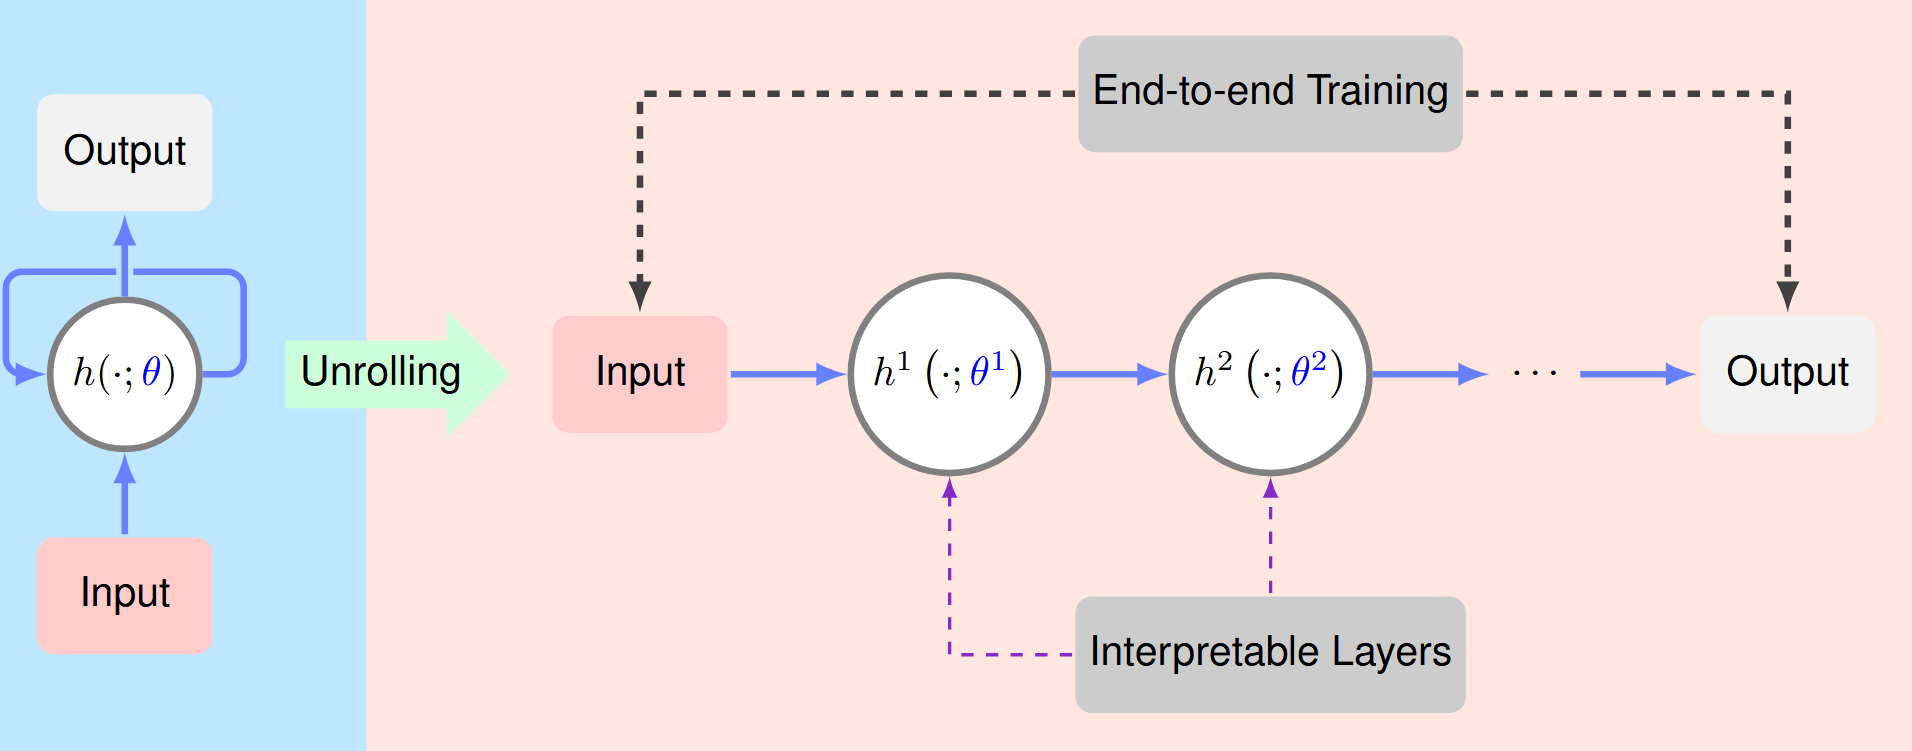
\includegraphics[width=\textwidth]{img/unrolling.png}
    \caption{
        \textbf{Tổng quan Algorithm unrolling:} cho một thuật toán lặp (bên trái), một neural network tương ứng (bên phải) có thể được tạo bằng cách ``trải'' các phép lặp $h$ ra. 
        Phép lặp $h$ 
        % (bên trái) 
        được thực thi với số lần hữu hạn, tương ứng với các lớp $h^1, h^2, \dots$ của mạng. Mỗi phép lặp $h$ phụ thuộc vào tham số $\theta$, và tham số này được 
        % truyền vào 
        biểu diễn bởi tham số của
        mạng dưới dạng $\theta^1, \theta^2, \dots$. Thay vì phải xác định các tham số một cách thủ công trong thuật toán lặp, ta học $\theta^1, \theta^2, \dots$ trực tiếp từ quá trình huấn luyện mô hình. Bằng cách này, mạng có thể đạt được hiệu suất tốt hơn so với thuật toán lặp ban đầu. Ngoài ra, các lớp của mạng được kế thừa tính diễn giải (interpretability) một cách tự nhiên từ quá trình lặp.
        Các tham số có thể học được có màu xanh.
        (được trích dẫn từ~\cite{monga2021unroll})
    }
    \label{fig:unrolling}
\end{figure}
